\documentclass[9pt,aspectratio=169]{beamer}
\usetheme{VK}

\usepackage{dsfont}
\usepackage{bm}
\usepackage{xunicode}
\usepackage{xltxtra}
\usepackage{xecyr}

\usepackage{tikz}
\usetikzlibrary{angles,quotes}

\usepackage{mwe}
\usepackage{multirow}

\usepackage{csquotes}
\usepackage[style=verbose-ibid,backend=bibtex]{biblatex}
\bibliography{references}

\date[]{}
\title[]{Название моего доклада}
\author[]{Иван Иванов}

\AtEndDocument{\usebeamertemplate{endpage}}

\begin{document}
\maketitle

\section{About}
\begin{frame}{Данные}
    
    \begin{columns}
    \column{0.3\textwidth}
        Уже похоже на нужные нам данные
    \column{0.5\textwidth}
        \begin{tabular}{l l}
            \dblock{160 GB}{Логов активности} & \dblock{97M}{Пользователей} \\[2cm]
            \dblock{3M}{Сообщест} & \dblock{13B}{Сессий}
        \end{tabular}
    \end{columns}
    
\end{frame}

\begin{frame}{Problem Formulation}
    \framesubtitle{Exact k-NN (Survey~\autocite{bhatia2010survey})}
    
    \ddef{Exact k-NN}{
        \textit{
        Given $(\mathcal{X}, \rho)$ - metric space, $X \subseteq \mathcal{X}$ - set of $n$ points and $q \in \mathcal{X}$ - query point, task of Exact k-NN is to find a set $kNN(q) \subseteq X $ such that $|kNN(q)| = k$ and
        \begin{equation*}
            \forall x \in kNN(q) \; \forall x' \in X \setminus kNN(q) \; \left( \rho(q, x) \leq \rho(q, x') \right)
        \end{equation*}
        }
    }
    \pause
    Examples of spaces
    \begin{itemize}
        \item $(\mathbb{R}^d, \| \cdot \|_2)$ --- Euclidian space
        \item $\left(\mathbb{R}^d,\arccos\frac{\langle \vecx, \vecy \rangle}{\| \vecx \| \cdot \| \vecy \|}\right)$ --- $\mathbb{R}^d$ with cosine distance
        \item $\ldots$
    \end{itemize}
    
\end{frame}

\begin{frame}
    \frametitle{Part I}
    \framesubtitle{Tools and Systems for Big Data Storage and Processing}
    
    \begin{minipage}{0.5\textwidth}
        \setbeamertemplate{enumerate items}{\raisebox{-0.2em}{\scalebox{1.3}{\circled{\color{white}\insertenumlabel}}}}
        \begin{enumerate}
            \itemsep1.3em
            \item Hadoop and MapReduce
            \item Apache Spark
            \item Spark SQL
        \end{enumerate}
    \end{minipage} \hfill
    \begin{minipage}{0.49\textwidth}
        \begin{figure}
            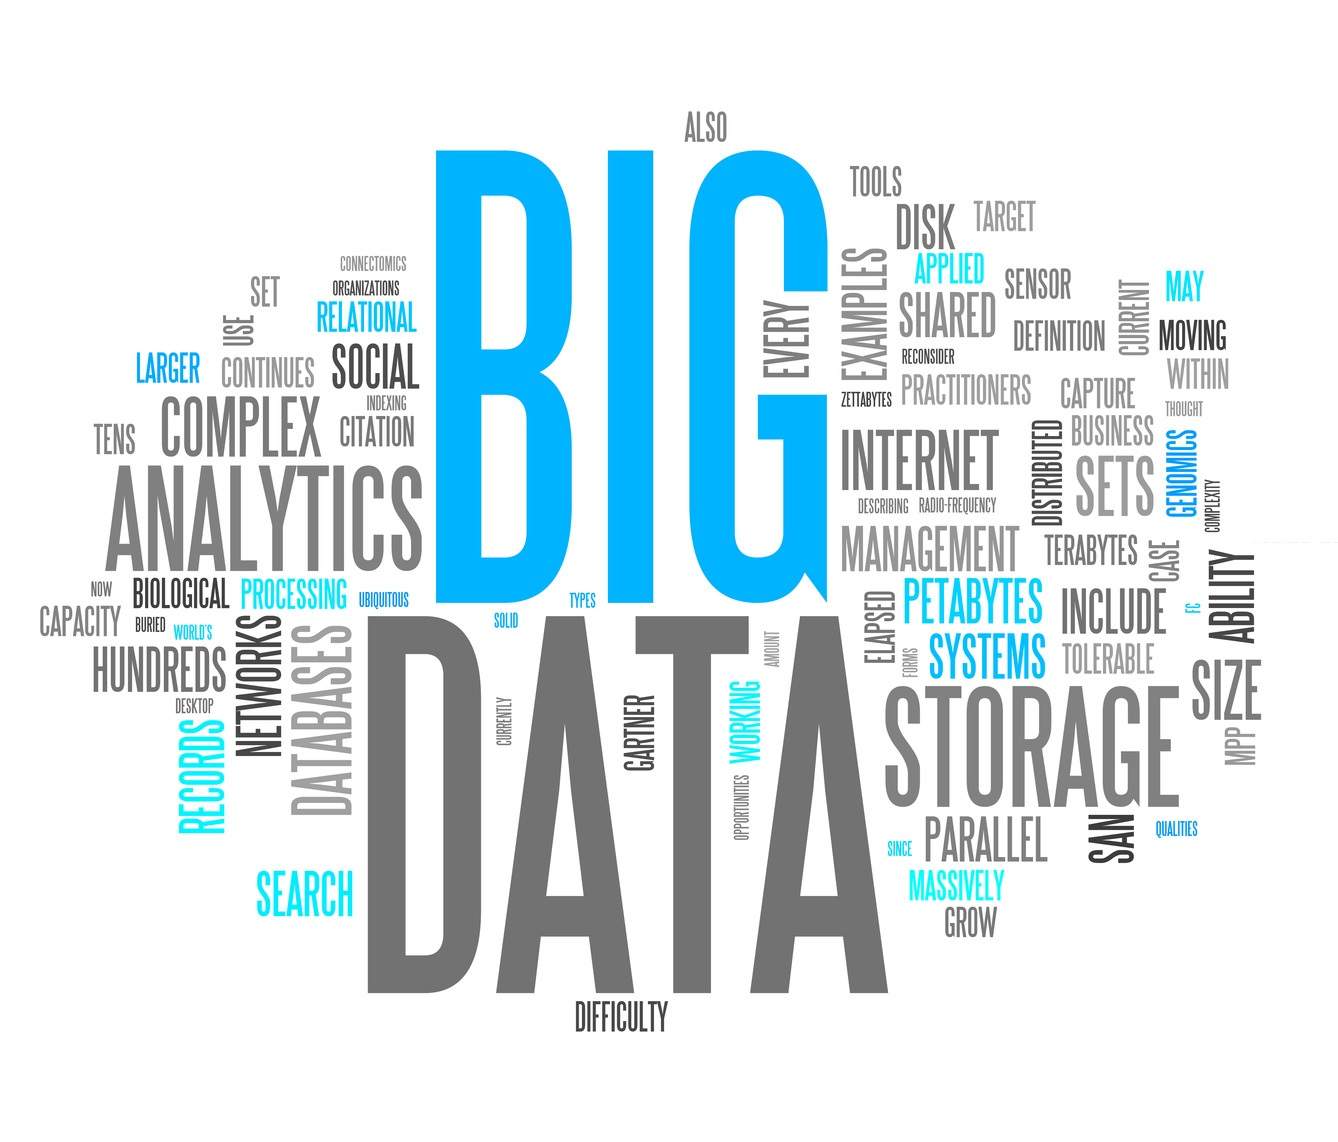
\includegraphics[width=1.0\linewidth]{images/big_data_image.jpg}
        \end{figure}
    \end{minipage}
    
\end{frame}

\section{Введение}
\subsection{Мотивация}
\begin{frame}
    \frametitle{Ключевые особенности}
    
    \dbox{
    \setbeamertemplate{itemize items}{\raisebox{-0.2em}{\scalebox{1.2}{\circledmark{}}}}
    \begin{itemize}
        \itemsep1.3em
        \item Большое количество данных и признаков ($ > 10^6 $)
        \item Сильно разряженные данные
        \item Категориальные признаки большой размерности
    \end{itemize}
    }
\end{frame}

\section{Программа}
\subsection{Лекции}
\begin{frame}{Конференции}
    \begin{center}
        \begin{tabular}{l l l}
            \dblocksep{KDD}{Knowledge Discovery and Data Mining} & \dblocksep{RECSYS}{Recommender System Conference} & \dblocksep{WWW}{World Wide Web Conference}
        \end{tabular}
    \end{center}

\end{frame}

\end{document} 